\documentclass[10pt]{amsart}
\usepackage[a4paper,margin=22mm]{geometry}
\usepackage[no-math]{fontspec}
\setmainfont{Latin Modern Roman}[SmallCapsFont={lmromancaps10-regular.otf}]
\usepackage{amsmath,amssymb,amsthm,mathtools,hyperref,graphicx,float}
\usepackage[shortlabels]{enumitem}
\emergencystretch=3em
\newtheorem{theo}{Theorem}[section]
\newtheorem{lemm}[theo]{Lemma}
\newtheorem{prop}[theo]{Proposition}
\newtheorem{coro}[theo]{Corollary}
\theoremstyle{definition}
\newtheorem{defi}[theo]{Definition}
\newtheorem{rema}[theo]{Remark}
\newtheorem{exam}[theo]{Example}
\usepackage{mathrsfs}

\DeclareMathOperator{\Gr}{Gr}
\newcommand{\Lm}{\Lambda}


%%%%%%%%% a placer avant \begin{document}


%%%%%%%%%%%%%%%%%%%%%%%%%%%%%%%%%%%%%
\newcommand*{\mk}{\mkern -1mu}
\newcommand*{\Mk}{\mkern -2mu}
\newcommand*{\mK}{\mkern 1mu}
\newcommand*{\MK}{\mkern 2mu}

\hypersetup{urlcolor=purple, linkcolor=blue, citecolor=red}


\newcommand*{\romanenumi}{\renewcommand*{\theenumi}{\roman{enumi}}}
\newcommand*{\Romanenumi}{\renewcommand*{\theenumi}{\Roman{enumi}}}
\newcommand*{\alphenumi}{\renewcommand*{\theenumi}{\alph{enumi}}}
\newcommand*{\Alphenumi}{\renewcommand*{\theenumi}{\Alph{enumi}}}
\title[Symmetric weak separation and plabic face labels]{Inclusion-maximal symmetric weakly separated collections in type-C positroids are symmetric reduced plabic face-label collections}
\author{Rachel Karpman}
\date{Algebraic Combinatorics3(6)(2020),1401–1416; DOI10.5802/alco.145}
\hypersetup{hidelinks}
\begin{document}
\maketitle
\setcounter{section}{1}
\section{Background}
\label{back}
\subsection{Intervals, subsets, and cyclic order.}

For natural numbers $k \leq m$, let $[m]$ denote the set $\{1,2,\ldots,m\}$, and let $\binom{[m]}{k}$ be the set of all $k$-element subsets of $[m]$. For $a \in [m]$, let $\leq_a$ denote the cyclic shift of the usual linear order on $m$ given by 
 
\begin{equation}
	a < a + 1 < \cdots < m < 1 < \cdots < a-1.
\end{equation}

We extend this to a partial order on $\binom{[m]}{k}$ by setting $I \leq_a J$ for
\[I = \{i_1 <_a i_2 <_a \cdots <_a i_k\}\]
\[J = \{j_1 <_a j_2 <_a \cdots <_a j_k\}\]
if $i_{\ell} \leq_a j_{\ell}$ for all $\ell \in [k]$.
For $a = 1$, this is the usual Gale order on $\binom{[m]}{k}$.
 
For $a,b \in [m]$, we define the \emph{cyclic interval} $[a,b]^{cyc}$ by

\begin{equation}
	[a,b]^{cyc} = \begin{cases}
	\{a,a+1,\ldots,b\} & a \leq b\\
	\{a,a+1,\ldots,n-1,n,1 \ldots,b\} & a > b
	\end{cases}.
\end{equation} 

Note that if the elements of $[m]$ are arranged clockwise around a circle, then elements of $[a,b]$ are consecutive. We say a sequence $a_1,a_2,\ldots,a_{\ell}$ of elements of $[m]$ is \emph{cyclically ordered} if, when the integers $1$ to $m$ are arranged clockwise around a circle, the terms $a_i$ appear in clockwise order.

Fix $n \in \mathbb{N}$. For $i \in [2n]$, let $i' = 2n - i + 1$. For each $I \in \binom{[2n]}{n}$, we define $\bar{I}$ to be the set 
\begin{equation}
	\bar{I} = [2n] \setminus \{i' \mid i \in I\}.
\end{equation} 

\subsection{Positroids in types A and C}

We realize the \emph{Grassmannian} $\Gr(k,m)$ as the space of $k \times m$ matrices, modulo row operations; a matrix corresponds to the span of its rows. The $k \times k$ minors of a matrix representative give homogeneous coordinates on $\Gr(k,m)$, called \emph{Pl{\"u}cker coordinates}. For $I \in \binom{[n]}{k}$, let $\Delta_I$ represent the determinant of the matrix minor with columns indexed by $I$.

The \emph{totally nonnegative Grassmannian} $\Gr_{\geq 0}(k,m)$ is the subset of $\Gr(k,m)$ where all Pl{\"u}cker coordinates are nonnegative real numbers, up to multiplication by a common scalar. For a point $P \in \Gr(k,m)$, the set 
\[
\mathcal{M} = \left\{I \in \binom{[m]}{k} \mathrel{\Bigg|} \Delta_I(P) \neq 0\right\}
\]
is called the \emph{matroid} of $P$. If $P$ is a point in $\Gr_{\geq 0}(k,m)$, the matroid of $P$ is a \emph{positroid}. The subset of $\Gr_{\geq 0}(k,m)$ consisting of all points with positroid $\mathcal{M}$ is a \emph{positroid cell}. Remarkably, positroid cells stratify $\Gr_{\geq 0}(k,m)$, and each positroid cell is homeomorphic to a ball~\cite{Pos06}. 

The positroid stratification of $\Gr_{\geq 0}(k,m)$ extends naturally to a stratification of the entire Grassmannian $\Gr(k,m)$ by \emph{positroid varieties}, which has nice geometric and combinatorial properties. For $P \in \Gr(k,m)$, there is a unique smallest positroid $\mathscr{P}$ which contains the matroid $\mathcal{M}$ of $P$; we call $\mathscr{P}$ the \emph{positroid} of $P$. We have $\mathscr{P}$ equal to $\mathcal{M}$ if $P \in \Gr_{\geq 0}(k,m)$; otherwise $\mathscr{P}$ is strictly larger than $\mathcal{M}$. The \emph{positroid variety} $\Pi$ corresponding to a positroid $\mathscr{P}$ is the set of all points in $\Gr(k,m)$ with positroid $\mathscr{P}$, and the totally nonnegative part of $\Pi$ is the positroid cell corresponding to $\mathscr{P}$. For details, see~\cite{KLS13}.

In~\cite{Kar18}, the author extends Postnikov's theory of total nonnegativity to the \emph{Lagrangian Grassmannian} $\Lm(2n)$, the parameter space of maximal isotropic subspaces with respect to a symplectic bilinear form. Concretely, we realize $\Lm(2n)$ as the subvariety of $\Gr(n,2n)$ which is cut out by the linear relations
\begin{equation}
\label{linear} \left\{\Delta_I = \Delta_{\bar{I}} \mathrel{\Bigg|} I \in \binom{[2n]}{n} \right\}.\end{equation} 
The \emph{symmetric part} of any $\Pi \subseteq Gr(n,2n)$ is the set-theoretic intersection of $\Pi$ with $\Lm(2n)$; that is, the subset of $\Pi$ where the relations~\eqref{linear} hold. 
 
The \emph{totally nonnegative} part of $\Lm(2n)$, denoted $\Lm_{\geq 0}(2n)$, is the subset of $\Lm(2n)$ where all Pl{\"u}cker coordinates are positive. A positroid cell (respectively, variety) is \emph{type C} if its symmetric part is nonempty. The symmetric part of a type C positroid cell is a \emph{totally nonnegative cell} in $\Lm_{\geq 0}(2n)$. Totally nonnegative cells form a stratification of $\Lm_{\geq 0}(2n)$, analogous to the positroid stratification, which extends naturally to a stratification of $\Lm(2n)$ by the symmetric parts of type C positroid varieties. In particular, the symmetric part of $\Pi$ is nonempty if and only if the intersection of $\Pi$ with $\Gr_{\geq 0}(n,2n)$ is a totally nonnegative cell in $\Lm_{\geq 0}(2n)$. For details, see~\cite{Kar18}. 

\subsection{Grassmann necklaces and decorated permutations}

In this section, we discuss two families of combinatorial objects which are in bijection with positroids. All of these definitions and results, as well as many additional details, can be found in~\cite{Pos06}.

\begin{defi}
A \emph{Grassmann necklace} of type $(k,m)$ is a sequence
$\mathcal{I} = (I_1,\ldots,I_m)$ of elements of $\binom{[m]}{k}$ such that $I_{i+1}$ contains $I_i \backslash \{i\}$ for all $i \in [m]$, where indices are taken modulo $m$.
\end{defi}

Note that if $i \not\in I_{i}$, we must have $I_{i+1} = I_i$. 
For a Grassmann necklace $\mathcal{I}$, define
\[\mathcal{M}_{\mathcal{I}} \coloneqq \left\{%\left.
J \in \binom{[m]}{n} \mathrel{\Bigg|} J \geq_i I_i \text{ for all }i \in [m]\right\}.\]
Remarkably, $\mathcal{M}_{\mathcal{I}}$ is a positroid, with $\mathcal{I} \subseteq \mathcal{M}_{\mathcal{I}}$, and every positroid arises uniquely in this way. 

\begin{defi}
A \emph{decorated permutation} is a permutation $f \in S_m$, with fixed points colored black or white. 
\end{defi}

To obtain a Grassmann necklace from a decorated permutation $f$, for each $a \in [m]$,~let
\[I_a = \{i \in [m] \mid i \leq_a f^{-1}(i) \text{ or $i$ is a white fixed point of $f$} \}.\]
Then $\mathcal{I} = (I_1,\ldots,I_m)$ is a Grassmann necklace, and this construction gives a bijection from Grassmann necklaces to decorated permutations. We say $f$ has type $(k,m)$ if the associated Grassmann necklace has type $(k,m)$.

\begin{defi}[{\cite[Section 17]{Pos06}}] For $i,j \in [m]$, we say that $(i,j)$ forms an \emph{alignment} of the decorated permutation $f$ if the numbers $i$, $f(i)$, $f(j)$ and $j$ appear in cyclic order, and are all distinct.
\end{defi}

Note that the order of $i$ and $j$ matters for this definition; if $(i,j)$ is an alignment, it is not the case that $(j,i)$ is also an alignment.

\subsection{Plabic graphs}

A \emph{plabic graph} is a planar graph embedded in a disk, with each vertex colored black or white. The boundary vertices are numbered $1,2,\ldots,n$ in clockwise order, and all boundary vertices have degree one. We call the edges adjacent to boundary vertices \emph{legs} of the graph. 

Postnikov defines a collection of paths and cycles in $G$, called \emph{trips}, as follows~\cite{Pos06}. Start by traversing a leg of the graph, starting on the boundary, then proceed according to the \emph{rules of the road}: turn (maximally) left at every white internal vertex, and (maximally) right at every black internal vertex. Continuing in this fashion, we eventually reach a boundary vertex, at which point the trip ends. See Figure~\ref{trip} for an example. We repeat this process for every boundary vertex of the graph.

\begin{figure}[ht]
\centering
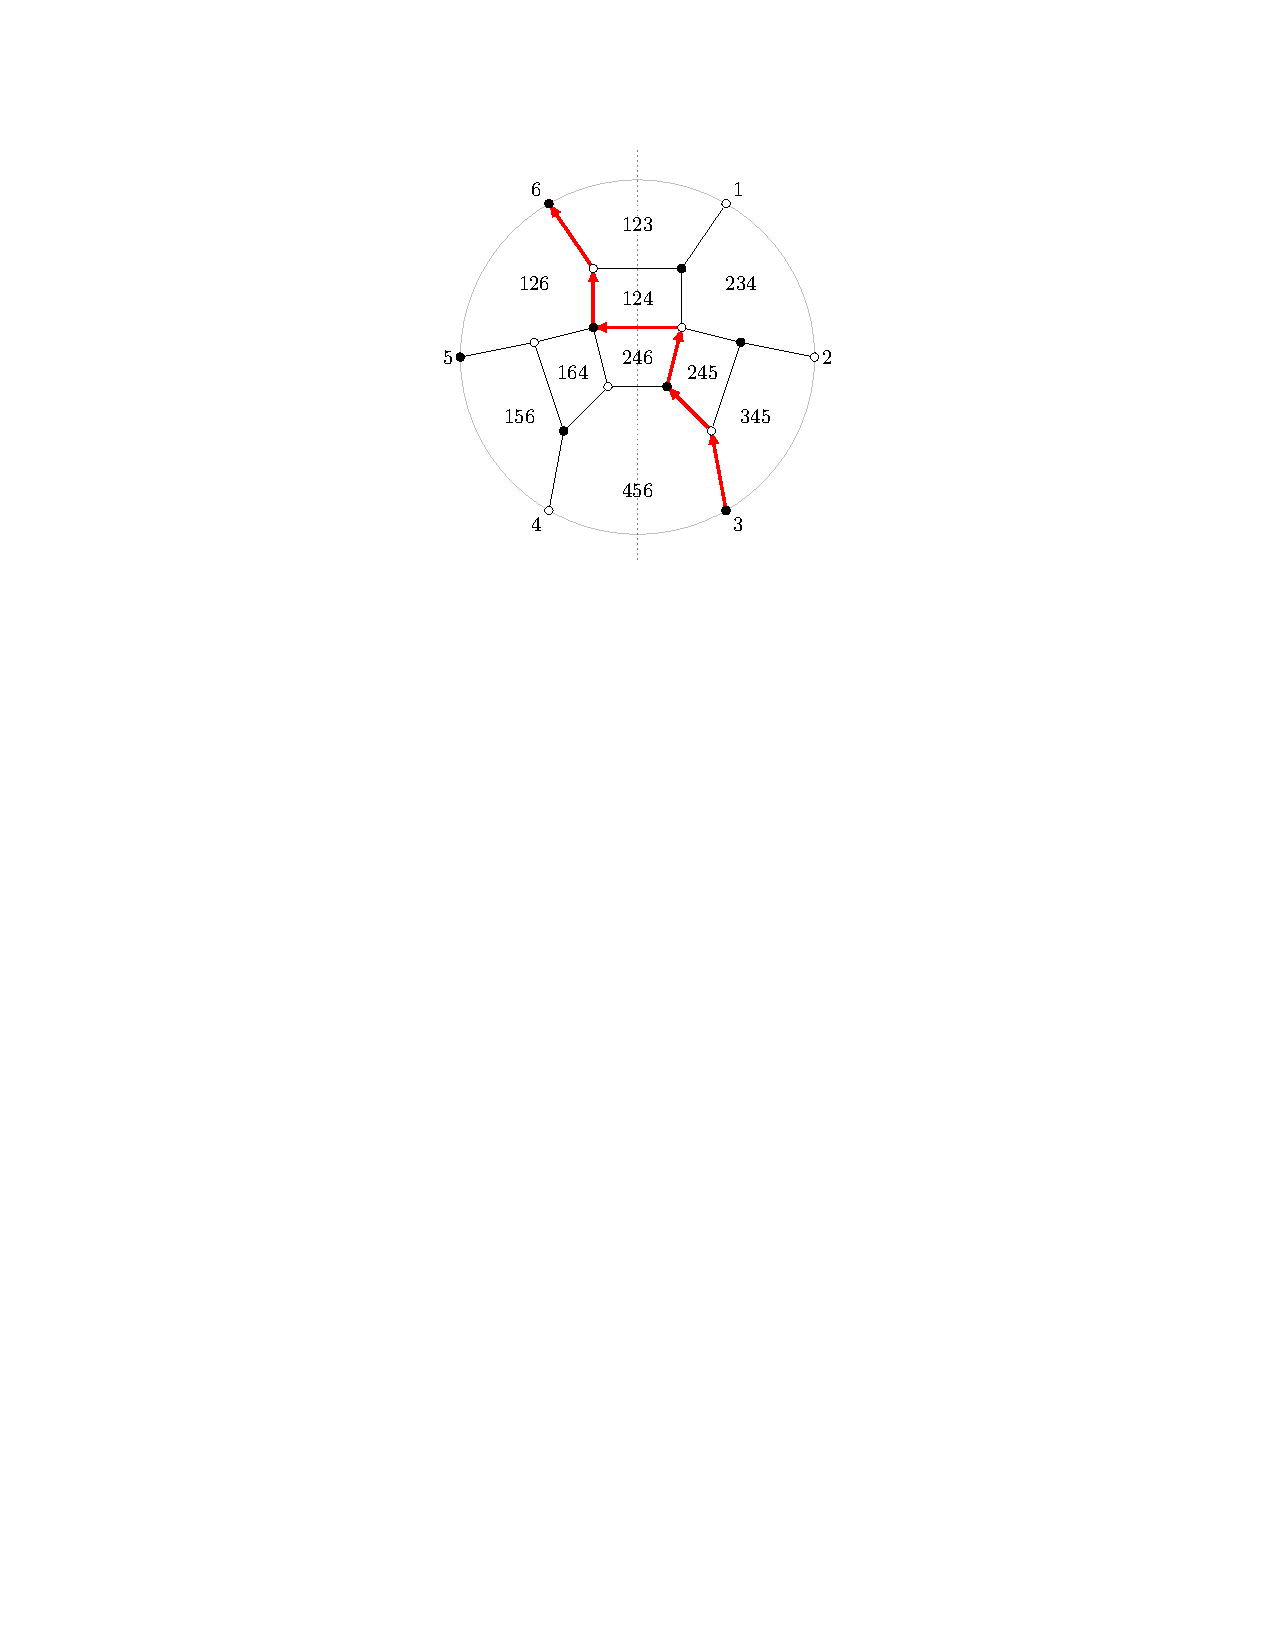
\includegraphics[trim={2in 7.25in 2in 1in},clip]{Figures/symmetric_36.pdf}

\caption{A plabic graph with face labels. Arrows show the trip from $3$ to $6$.}
\label{trip}
\end{figure}

In the remainder of this paper, we restrict our attention to \emph{reduced} plabic graphs. Postnikov defined reduced plabic graphs in terms of certain local transformations, and gave a criterion for a plabic graph $G$ to be reduced~\cite[Section 13]{Pos06}. We take this criterion as the \emph{definition} of a reduced graph.

\begin{defi}
\label{def_red}
A plabic graph $G$ is \emph{reduced} if it satisfies the following criteria:
\begin{enumerate}
\item The union of the trips defined above covers each edge of the graph exactly twice, once in each direction.
\item $G$ has no leaves, except perhaps some which are adjacent to boundary vertices. 
\item \label{norep} No trip uses the same edge twice, once in each direction, unless that trip starts (and ends) at a boundary vertex connected to a leaf.
\item No trips $T_1$ and $T_2$ share two edges $e_1$ and $e_2$ such that $e_1$ comes before $e_2$ in both trips. 
\end{enumerate}
\end{defi}

Given a plabic graph $G$ with $m$ boundary vertices, we define the \emph{trip permutation} 
$f$
of $G$ by setting 
\begin{math} f(a) = b\end{math}
if the trip that starts at boundary vertex $a$ ends at boundary vertex $b$. Notice that if $f$ has a fixed point at $a$, then $G$ must have a boundary leaf at $a$, to avoid violating Condition~\ref{norep} above. Hence we can define the \emph{decorated trip permutation} of $G$ by coloring each fixed point of $f$ either black or white, depending on the color of the corresponding boundary leaf. 


\subsection{Face labels for plabic graphs.}
\label{faces}

Let $G$ be a reduced plabic graph with $m$ boundary vertices, and suppose the decorated permutation $f$ of $G$ has type $(k,m)$. 
Let $\mathcal{M} \subseteq \binom{[m]}{k}$ be the positroid associated to $f$. 
For each $i \in [m]$, label each face $F$ of $G$ with an $i$ if $F$ is to the \emph{left} of the trip which \emph{ends} at boundary vertex $i$. See Figure~\ref{trip} for an example. Once all trips are accounted for, each face is labeled with an element of $\binom{[m]}{k}$, which is contained in $\mathcal{M}$~\cite{JS06}. Moreover, the faces adjacent to the boundary of $G$ are labeled with the elements of the Grassmann necklace $\mathcal{I}=(I_1,\ldots,I_n)$ of $\mathcal{M}$ in clockwise order; the boundary face between leg $i-1$ and leg $i$ has label $I_i$ where indices are taken modulo $m$~\cite{OPS15}. The Pl{\"u}cker coordinates corresponding to minors with columns indexed by face labels of $G$ give homogeneous coordinates on an open, dense subset of the positroid variety $\Pi$ of $\mathcal{M}$~\cite{MS17}.

More precisely, let $\mathcal{F}$ denote the set of face labels of $G$, and let $\Pi_{\mathcal{F}}$ be the subset of $\Pi$ where the Pl{\"u}cker coordinates indexed by elements of $\mathcal{F}$ are nonzero. A \emph{face weighting} of $G$ is an assignment of a number, or \emph{weight}, to each face of $G$. Let $(\mathbb{C}^{\times})^{\mathcal{F}}/\mathbb{C}^{\times}$ denote the space of nonzero face weights of $G$, modulo multiplication by a common scalar. Then by~\cite[Theorem 7.1]{MS17}, there is an isomorphism
\[\mathbb{F}: \Pi_{\mathcal{F}} \rightarrow (\mathbb{C}^{\times})^{|\mathcal{F}|}/\mathbb{C}^{\times}\]
which takes a point $P \in \Pi_{\mathcal{F}}$ and labels each face of $G$ with the corresponding Pl{\"u}cker coordinate of $P$. 

We note further that $\mathbb{F}$ maps the totally nonnegative part of $\Pi$, which is a positroid cell, isomorphically onto the space of positive face weightings of $G$. This is implicit, for example, in the statement of Theorem 7.1 from~\cite{MS17}, as the maps $\overleftarrow{\mathbb{M}}$, $\overrightarrow{\mathbb{M}}$, $\overleftarrow{\partial}$ and $\overrightarrow{\partial}$ referenced in the theorem statement take positive edge weightings to positive face weightings and vice versa. For details, see~\cite[Section 5.3--5.4]{MS17}.

\subsection{Symmetric plabic graphs}

For $n \in \mathbb{N}$, a plabic graph with $2n$ boundary vertices is a \emph{symmetric plabic graph} 
if it is symmetric as an uncolored network with respect to reflection through a distinguished diameter which intersects the boundary of the disk between vertices $2n$ and $1$, and between vertices $n$ and $n+1$; and each vertex and its mirror image have opposite colors. By convention, the line of reflection runs vertically down the center of the graph, with vertices $1$ and $2n$ appearing above vertices $n$ and $n+1$, respectively. The plabic graph in Figure~\ref{trip} is symmetric. 

\begin{theo}[\cite{KS18}]
Let $\mathcal{M}$ be a positroid of type $(n, 2n)$. Then the following are equivalent:
\begin{enumerate}
\item The positroid cell corresponding to $\mathcal{M}$ has nonempty intersection with $\Lm(2n)$.
\item For all $i \in [2n]$, the decorated permutation $f$ of $\mathcal{M}$ satisfies 
\[f(i') = (f(i))',\]
and if $i$ and $i'$ are both fixed points of $f$, then exactly one of $i,i'$ is white and the other is black.
\item For all $i \in [2n]$, the Grassmann necklace $\mathcal{I}$ of $\mathcal{M}$ satisfies 
\[I_{i'} = \overline{I_{(i + 1)}}.\]
\item There is a symmetric plabic graph with associated positroid $\mathcal{M}.$
\end{enumerate}
\end{theo}

\begin{defi} We say a decorated permutation, Grassmann necklace, or positroid is type C if the associated positroid cell has nonempty intersection with $\Lm(2n)$.
\end{defi}
 
\subsection{Weakly separated collections and plabic tilings}

The following definitions, with additional details, may be found in~\cite{OPS15}.

\begin{defi}
Let $I, J \in \binom{[m]}{k}$.
We say $I$ and $J$ are \emph{weakly separated} if there do not exist $a,b,a',b'$, cyclically ordered such that $a,a' \in I \backslash J,$ and $b, b' \in J \backslash I$. Equivalently, $I$ and $J$ are weakly separated if, when the elements of $[m]$ are arranged in a circle, there is a chord separating the elements of $J \backslash I$ from the elements of $I \backslash J$.
\end{defi}

\begin{defi}Let $\mathcal{C} \subseteq \binom{[m]}{k}$. Then $\mathcal{C}$ is a \emph{weakly separated collection} if for each $I, J \in \mathcal{C}$, the sets $I$ and $J$ are weakly separated. A weakly separated collection is \emph{maximal by inclusion} if it is not contained in any larger weakly separated collection in $\binom{[m]}{k}$; equivalently, if for every $I \in \binom{[m]}{k}$ with $I \not\in \mathcal{C}$, there is some $J \in \mathcal{C}$ such that $I$ and $J$ are \emph{not} weakly separated.
\end{defi}

\begin{defi}
Let $\mathcal{M}$ be a positroid with Grassmann necklace $\mathcal{I}$, and let $\mathcal{C}$ be a weakly separated collection in $\binom{[m]}{k}$. Then $\mathcal{C}$ is a \emph{weakly separated collection in $\mathcal{M}$} if $\mathcal{I} \subseteq \mathcal{C} \subseteq \mathcal{M}$. A maximal weakly separated collection in $\mathcal{M}$ is \emph{maximal by inclusion} if it is not contained in any larger weakly separated collection in $\mathcal{M}$.
\end{defi}


Our goal is to prove a symmetric version of following theorem.

\begin{theo}[\cite{OPS15}]
\label{ops_main}
Let $\mathcal{M}$ be a positroid, and let $C$ be a weakly separated collection in $\mathcal{M}$. Then the following are equivalent.
\begin{enumerate}%[(1)]
\item $\mathcal{C}$ is maximal by inclusion.
\item $\mathcal{C}$ is maximal by size among all weakly separated collections in $\mathcal{M}$.
\item $\mathcal{C}$ is the set of face labels of a reduced plabic graph with associated positroid~$\mathcal{M}$.
\end{enumerate}
\end{theo}

\subsection{Plabic tilings}

Let $\mathcal{M}$ be a positroid, and let $\mathcal{C}$ be a maximal weakly separated collection in $\mathcal{M}$. Oh, Postnikov and Speyer construct an abstract CW-complex called a \emph{plabic tiling} with vertices indexed by $\mathcal{C}$, then give an embedding of the complex into $\mathbb{R}^2$. We proceed directly to a description of the embedded tiling, which is all that we need. See~\cite[section 9]{OPS15} for details.

Fix $m$ points $v_1,\ldots,v_m$ which form the vertices of a convex $m$-gon in $\mathbb{R}^2$, numbered in clockwise order. We construct a two-dimensional CW-complex $\Sigma(\mathcal{C})$ whose vertices are the points 
\[\left\{v_I \coloneqq \sum_{i \in I} v_i \mathrel{\Bigg|} I \in \mathcal{C}\right\}.\]

For each $(k-1)$-element subset $K$ of $\binom{[m]}{k}$, the \emph{white clique} corresponding to $K$ is the set 
\[
\{I \in \mathcal{C} \mid I = K \cup \{a\} \text{ for some } a \in [m]\}.
\]

For each $(k+1)$-element subset $L$ of $\binom{[m]}{k}$, the \emph{black clique} corresponding to $L$ is \[\{I \in \mathcal{C} \mid I = L \backslash \{b\} \text{ for some } b \in L\}.\]

A clique is \emph{non-trivial} if it contains three or more vertices. The points $v_I$ corresponding to elements of a non-trivial clique are the vertices of a convex polygon in $\mathbb{R}^2$. We take these polygons to be the two-dimensional cells of $\Sigma(\mathcal{C})$, and the edges of these polygons to be one-dimensional cells.
We also add an edge from $v_I$ to $v_J$ for any $I, J \in \mathcal{C}$ such that all of the following hold:
\begin{enumerate}
\item $I = (J \backslash \{a\}) \cup \{b\}$ for some $a, b \in [m]$.
\item $\{I,J\}$ is the (trivial) white clique of $I \cap J.$
\item $\{I, J\}$ is also the (trivial) black clique of $I \cup J$.
\end{enumerate}

\begin{rema}
\label{mostly_same}
Let $I$ and $J$ be two elements of a weakly separated collection $\mathcal{C} \subseteq \binom{[m]}{k}$. If $I$ and $J$ are contained in the same clique in $\mathcal{C}$, then $I \cap J = k-1$. Indeed, if $I$ and $J$ are vertices of the same white clique, then there is some $(k-1)$-element set $K$ and some $a, b \not\in K$ such that $I = K \cup \{a\}$, $J = K \cup \{b\}$. Hence $I \cap J = K$ and the claim follows. If the clique is black, then there is some $(k+1)$-element set $L$ and some $a,b \in L$ such that $I = L \backslash \{a\},$ $J = L \backslash \{b\}$. So $I \cap J = L \backslash \{a,b\}$, and again the claim follows.

Note that if two vertices in a plabic tiling are adjacent, then they are contained in a common clique, and thus have all but one of their elements in common.
\end{rema}

This construction yields a connected CW-complex embedded in the plane. Remarkably, taking the planar dual of $\Sigma(\mathcal{C})$, and coloring each vertex according to the color of the corresponding face, we obtain a reduced plabic graph. For each $I \in \mathcal{C}$, Scott's construction assigns the label $I$ to the face of of the graph corresponding to $v_I$.
 
\begin{figure}[ht]
\centering
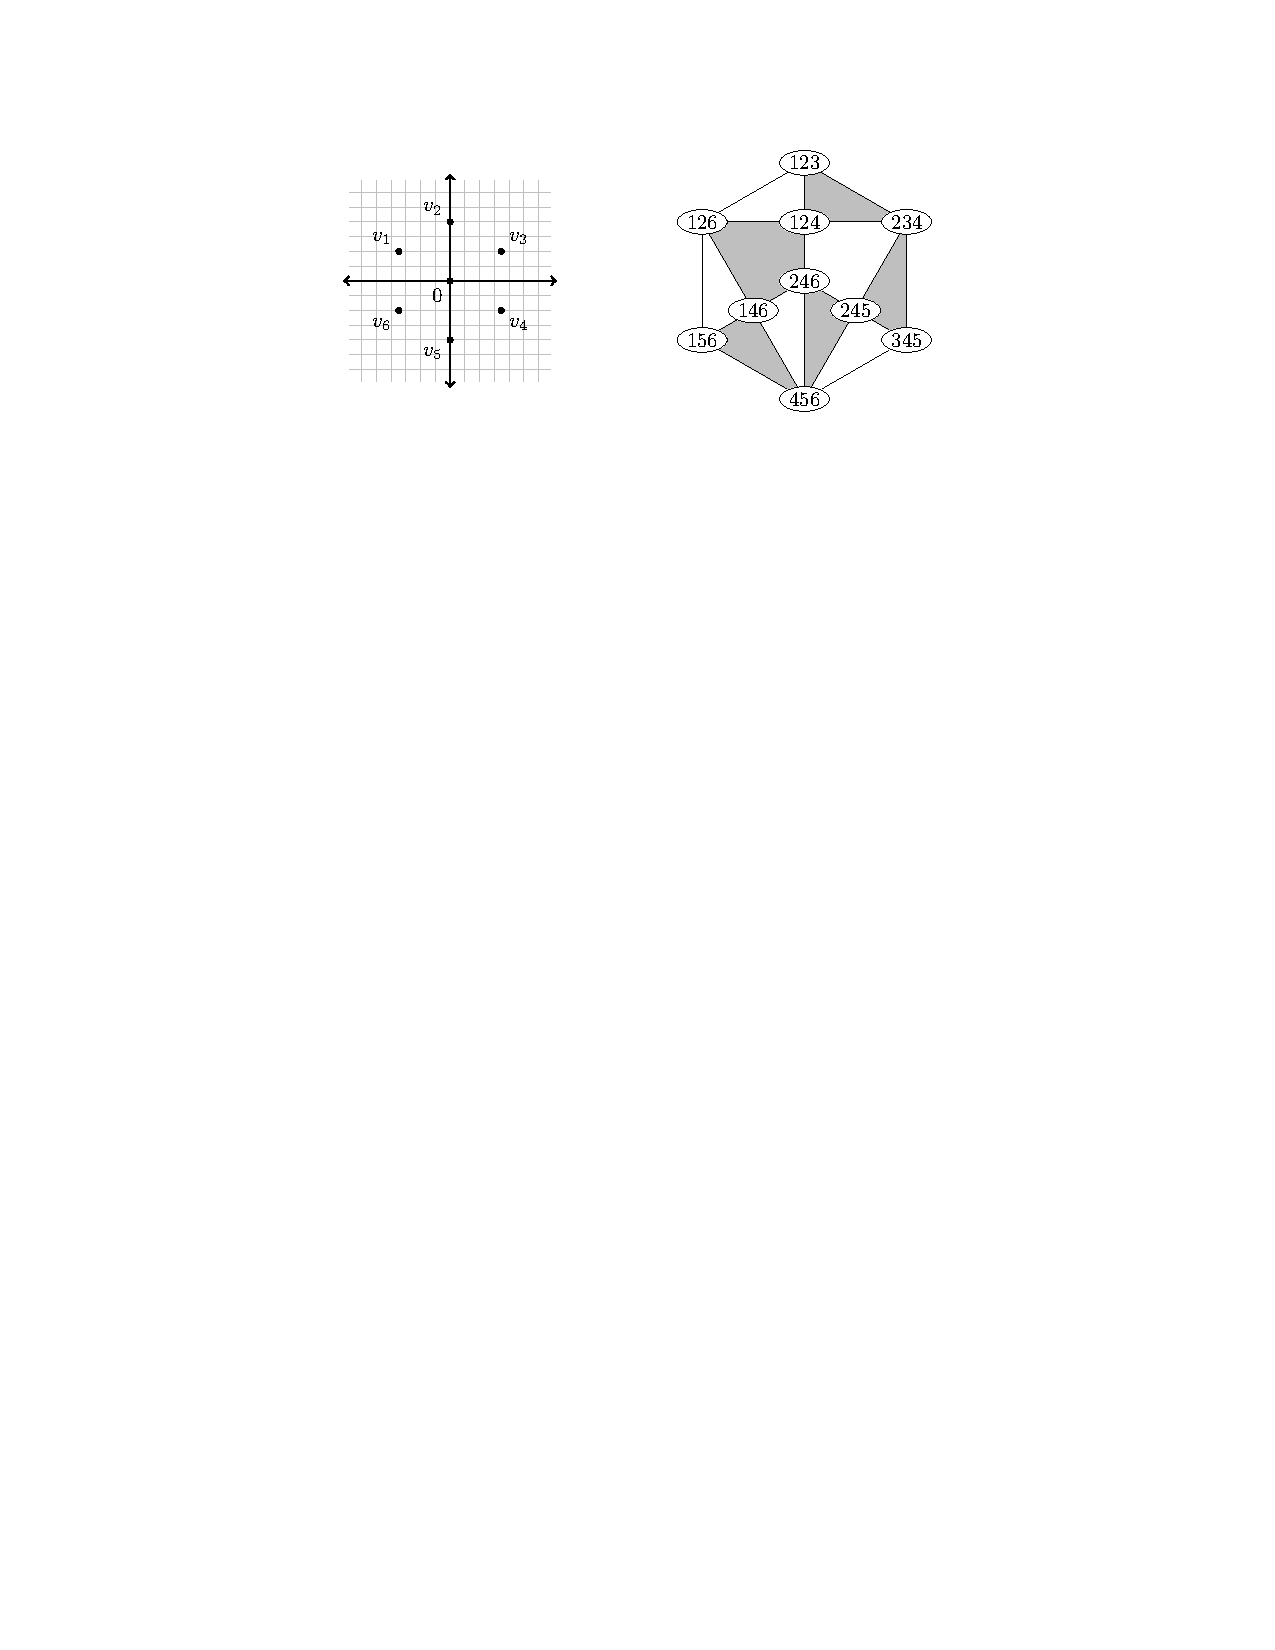
\includegraphics[trim={2in 8.25in 2in 1in},clip]{Figures/plabic_tiling.pdf}

\caption{A symmetric plabic tiling, defined using the points $v_1,\ldots,v_6$ at left. This tiling is dual to the graph in Figure~\ref{trip}.}
\label{numbers}
\end{figure}

Let $G$ be a plabic graph with a boundary leaf at $i \in [m]$. If the leaf $i$ is white, then $i$ is contained in every face label of $G$. If the leaf is black, then $i$ is contained in none of the face labels. Hence removing the boundary leaf at $i$ and re-indexing the boundary vertices has no effect on the combinatorial structure of the corresponding tiling, and we may safely reduce to the case of plabic graphs whose trip permutations are fixed-point free.

\section{Symmetric face labels and the Lagrangian Grassmannian}
\label{sym_face}

In this section, we prove that \emph{symmetric face weights} of a symmetric plabic graph give rational coordinates on the symmetric part of the associated positroid variety; and that positive, symmetric face weights give coordinates on the corresponding totally nonnegative cell in $\Lm(2n)$.

\begin{defi}We say a symmetric plabic graph has \emph{symmetric face weights} if each face has the same weight as its mirror image. A graph has \emph{positive} face weights if all of its face weights are positive, up to multiplication by a common nonzero scalar.
\end{defi}

\begin{lemm}\label{mirror}
Let $F$ be a face of a symmetric plabic graph $G$, and let $\overline{F}$ be its mirror image. Then if $F$ has label $I$, $\overline{F}$ has label $\overline{I}$.
\end{lemm}

\begin{proof}
Reflecting $G$ through the line of symmetry sends the trip ending at $i$ to the trip ending at $i'$ for all $i \in [2n]$. Hence $F$ is to the the left of the trip ending at $i$ if and only if $\overline{F}$ is to the \emph{right} of the trip ending at $i'$. The claim follows. \end{proof}



\begin{prop}
\label{sym_face_weights}
Let $\Pi$ be a positroid variety of type $C$ in $\Gr(n,2n)$, and let $G$ be a symmetric plabic graph for $\Pi$. Let $\Pi^C$ be the symmetric part of $\Pi$. Then restricting the face Pl{\"u}cker map $\mathbb{F}$ gives an isomorphism from an open, dense subset of $\Pi^C$ to the space of symmetric face weightings of $G$. Restricting further to the totally nonnegative part of $\Pi^C$, we obtain an isomorphism to the space of \emph{positive} symmetric face weightings of $G$.
\end{prop}

\begin{proof}
Let $\mathcal{F}$ and $\Pi_{\mathcal{F}}$ be defined as in Section~\ref{faces}, and let $\Pi_{\mathcal{F}}^C$ be the symmetric part of $\Pi_{\mathcal{F}}$. Then $\Pi^C_{\mathcal{F}}$ is an open subset of $\Pi^C$ which is nonempty, since in particular $\Pi^C_{\mathcal{F}}$ contains the totally nonnegative part of $\Pi^C$. Since $\Pi^C$ is an irreducible variety~\cite{Kar18}, it follows that $\Pi^C_{\mathcal{F}}$ is an open dense subset of $\Pi^C$.

Let $W$ denote the space of symmetric weights of $G$, modulo scaling. Clearly, $\mathbb{F}$ maps $\Pi_{\mathcal{F}}^C$ into $W$. Our task is to show that the map is surjective onto $W$. For this, note that $\mathbb{F}$ is a rational map which is regular on its domain of definition~\cite{MS17}. It follows that $\mathbb{F}$ maps $\Pi_{\mathcal{F}}^C$ isomorphically to a closed subvariety of $W$. Since $W$ is irreducible, it suffices to show that $\Pi_{\mathcal{F}}^C$ and $W$ have the same dimension.

Let $\ell=\dim(W)$. Identifying opposite pairs of faces in $G$, and subtracting one to account for scaling, we see that $\ell$ is one less than the number of faces of $G$ which either intersect the distinguished line of reflection, or lie strictly to its left. But this is the dimension of $\Pi_{\mathcal{F}}^C$, by results of~\cite[Section 5]{Kar18}. Hence the dimension of $\Pi_{\mathcal{F}}^C$ is precisely the dimension of $W$, proving the claim.

Next, we show that $\mathbb{F}$ induces an isomorphism from the totally nonnegative part of $\Pi_{\mathcal{F}}^C$ to the space of \emph{positive} symmetric weightings of $G$, modulo scaling. Recall that $\mathbb{F}$ restricts to a bijection from the totally nonnegative part of $\Pi$, which is contained in $\Pi_{\mathcal{F}}$, to the space of positive face weights, modulo scaling. Moreover, we have seen that $\mathbb{F}$ maps $\Pi_{\mathcal{F}}^C$ bijectively to $W$, the space of symmetric weightings, again modulo scaling. Hence restricting $\mathbb{F}$ to the totally nonnegative part of $\Pi_{\mathcal{F}}^C$ gives an isomorphism to the space of positive, symmetric weightings of $G$ modulo scaling, as desired. \end{proof}

We have shown that the face Pl{\"u}cker map $\mathbb{F}$ restricts to an isomorphism from a totally nonnegative cell in $\Lm(2n)$ to the space of positive, symmetric face weightings of a symmetric plabic graph. 
Note that since $\mathbb{F}$ is injective on $\Pi_{\mathcal{F}}$, the map $\mathbb{F}$ takes a point $P \in\Pi_{\mathcal{F}}^C$ to a \emph{positive} symmetric weighting of $G$ \emph{only} if $P$ is in the totally nonnegative part of $\Pi^C$.

A collection $\mathcal{C}$ of Pl{\"u}cker coordinates is a \emph{total positivity test} for $\Gr(k,m)$ if all elements of $\mathcal{C}$ are simultaneously positive \emph{only} for points in $\Gr_{> 0}(k,m)$.
Hence any maximal weakly separated collection gives a total positivity test for $\Gr(k,m)$, which is minimal by inclusion. Similarly, we may say a collection $\mathcal{C}$ of Pl{\"u}cker coordinates is a total positivity test for $\Lm(2n)$ if, whenever the element of $\mathcal{C}$ are simultaneously positive for $P \in \Lm(2n)$, we have $P \in \Lm_{>0}(2n)$. Proposition~\ref{faces} shows that we obtain a total positivity test for $\Lm(2n)$ from any symmetric plabic graph for $\Lm_{>0}(2n)$, by for example taking the labels of all faces which either intersect the distinguished diameter, or lie strictly to the left of it. 

\section{Symmetric weakly separated collections}
\label{sym_sep}

\begin{defi}
A weakly separated collection $\mathcal{C}$ is \emph{symmetric} if for all $I \in \mathcal{C}$, we have $\bar{I} \in \mathcal{C}$.
\end{defi}

Hence the face labels of a symmetric plabic graph form a symmetric weakly separated collection. In particular, if $\mathcal{I}=(I_1,\ldots,I_{2n})$ is a Grassmann necklace of type $C$, then the elements of $\mathcal{I}$ form a symmetric weakly separated collection, since we have $\overline{I_i} = I_{i' + 1}$ for each $i \in [2n]$, with indices taken modulo $2n$. Note that if $I$ is contained in a symmetric weakly separated collection, then $I$ and $\bar{I}$ must be weakly separated.

\begin{defi}
An element $I$ of $\binom{[2n]}{n}$ is \emph{admissible} if $I$ and $\bar{I}$ are weakly separated.
\end{defi} 

Let $I \in \binom{[2n]}{n}$. We say that $I$ has a \emph{full pair} at $\{a,a'\}$ if $a,a' \in I$; $I$ has a \emph{half pair} at
 $\{a,a'\}$ if exactly one of
 $\{a,a'\}$ is in $I$; and $I$ has an \emph{empty pair} at
 $\{a,a'\}$ if $a,a' \not\in I$. 
 For $a,b \in [n]$, we say the pair $\{a,a'\}$ is above $\{b,b'\}$ if $a < b$. Hence when $\{a,a',b,b'\}$ are drawn as boundary vertices of a plabic graph with our conventions, the elements of
 $\{a,a'\}$ indeed lie above the elements $\{b,b'\}$. 

\begin{lemm}
$I$ is admissible if and only if no full pair of $I$ has both an empty pair above it and an empty pair below it; and no empty pair has both a full pair above it and a full pair below it. 
\end{lemm}

\begin{proof}
Note that $\bar{I}$ is obtained from $I$ by replacing the full pairs of $I$ with empty pairs and vice versa. Hence $I \backslash \bar{I}$ is precisely the union of the full pairs of $I$, and $\bar{I} \backslash I$ is the union of the empty pairs of $I$. The lemma follows. \end{proof}

\begin{defi}An elements $I$ of $\binom{[2n]}{n}$ is \emph{pair-free} if $I$ has no full pairs, and consequently no empty pairs. 
\end{defi}

\begin{rema}
\label{I1_is_pair_free}
Pair-free elements will be important in the proof of our main result. Note that $\bar{I} = I$ if and only if $I$ is pair-free. For a Grassmann necklace $\mathcal{I}=(I_1,\ldots,I_{2n})$ of type $C$, we have $\overline{I_1} = I_{2n + 1} = I_1$
so $I_1$ is pair-free. 
By a similar argument, so is $I_{n + 1}.$
\end{rema}

\begin{lemm}\label{pairless}Let $\mathcal{M}$ be a positroid of type $C$, with trip permutation $f$. Let $\mathcal{J}$ be a set of pair-free elements contained in a weakly separated collection in $\mathcal{M}$. Then the following hold:
\begin{enumerate}
\item\label{lemm4.6_1} For $I \in \mathcal{J}$, if $\{a, f^{-1}(a)\} \subseteq [n]$ and $f^{-1}(a) > a$, then $a \in I$.
\item\label{lemm4.6_2} For $I \in \mathcal{J}$, if $\{a,f^{-1}(a)\} \subseteq [n]$ and $f^{-1}(a) < a$, then $a' \in I$.
\item\label{lemm4.6_3} For $I, J \in \mathcal{J}$, either $(I \cap [n]) \subseteq (J \cap [n])$, or $(J \cap [n]) \subseteq (I \cap [n])$.
\end{enumerate}
\end{lemm}

\begin{proof}
To prove~\eqref{lemm4.6_1}, observe that by symmetry, $(f^{-1}(a),f^{-1}(a'))$ is an alignment of~$f$. So by Corollary 11.4 in~\cite{OPS15}, if $I$ contained $a'$, then $I$ would necessarily contain $a$ as well, contradicting the fact that $I$ is pair-free. Hence $I$ must contain $a$, and not $a'$. The proof of~\eqref{lemm4.6_2} is analogous. For the last condition, let $I$ and $J$ be pair-free elements of $\binom{[2n]}{n}$. Suppose we have $a,b \in [n]$ such that $a \in I \backslash J$ and $b \in J \backslash I$. Then since $I$ and $J$ are pair-free, we have
$a' \in J \backslash I$ and $b' \in I \backslash J$. Without loss of generality, say $a < b$. Then
\[a < b < b' < a'.\]
Since $\{a,b'\} \in I \backslash J$ and $\{b,a'\} \in J \backslash I$, $I$ and $J$ are not weakly separated. The claim follows by contrapositive. 
\end{proof}

\begin{rema}
\label{explain_spine}
For $\mathcal{M}$ a positroid of type $C$ with decorated permutation $f$ and Grassmann necklace $\mathcal{I}= (I_1, I_2, \ldots, I_{2n})$, define the set
\begin{equation}
	S = \{a \in [n] \mid f^{-1}(a) > n\}.
\end{equation}
It follows from the definition of the Grassmann necklace that $S \subseteq I_1$, and that $I_{n+1}$ is obtained from $I_1$ by replacing $a$ with $a'$ for each $a \in S$.

Let $r = |S| + 1$. By Lemma~\ref{pairless}, a symmetric weakly separated collection $\mathcal{C}$ in $\mathcal{M}$ contains at most $r$ pair-free elements. If $\mathcal{C}$ contains $r$ pair-free elements, then they must be obtained by starting with $I_1$, and successively replacing $a$ with $a'$ for each $a \in S$ until we have $I_{n+1}$. Note that the elements of $S$ may or may not be replaced in increasing order.
\end{rema}

\begin{defi}
Let $\mathcal{M}$ be a positroid of type $C$ with Grassmann necklace $\mathcal{I}=\{I_1,\ldots,I_{2n}\}$ and decorated permutation $f$. Let $r$ be as in Remark~\ref{explain_spine}. We call a collection of pair-free elements $\mathcal{J} \subseteq \mathcal{M}$ a \emph{spine} if $|\mathcal{J}| = r$, and $\mathcal{J} \cup \{I_1,\ldots,I_{2n}\}$
is a weakly separated collection. 
\end{defi}

\begin{lemm}
\label{has_spine}
Let $\mathcal{C}$ be the set of face labels of a symmetric plabic graph $G$. Then~$\mathcal{C}$ contains a spine, which comprises the labels of the faces of $G$ that intersect the midline of the graph. 
\end{lemm}

\begin{proof}
Let $\mathcal{M}$, $\mathcal{I}$, and $f$ be the positroid, Grassmann necklace, and decorated permutation respectively of the symmetric plabic graph $G$. We first prove that no trip in $G$ crosses the distinguished diameter $d$ of the symmetric plabic graph more than once. To see this, let $T_1$ be a trip in $G$, and suppose $T_1$ crosses the midline twice: first at edge $e_1$ and next at edge $e_2$. With our conventions for symmetric plabic graphs, each edge which intersects the distinguished diameter $d$ of $G$ must be perpendicular to $d$. Suppose without loss of generality that $T_1$ traverses $e_1$ from left to right, and $e_2$ from right to left. 

By symmetry, there is a trip $T_2$ in $G$ which is obtained by reflecting $T_1$ through the line $d$. This implies that $T_2$ first crosses $e_1$ from right to left, and then crosses $e_2$ from left to right. Hence the pair of trips $T_1, T_2$ violate Condition~\eqref{norep} of Definition~\ref{def_red}. This is a contradiction, since the graph $G$ is assumed to be reduced. Hence each trip in $G$ crosses the diameter $d$ either once or not at all.

As in Remark~\ref{explain_spine}, let $S = \{a \in [n] \mid f^{-1}(a) > n\}$. Let $e$ be an edge of $G$ which crosses the midline of $d$, and again let $T_1$ and $T_2$ be the trips which pass through $e$. Suppose $T_1$ traverses $e$ from left to right, and $T_2$ traverses $e$ from right to left. Since $T_1$ crosses the midline exactly once, moving from left to right, it follows that $T_1$ ends at some $a \in [n]$ such that $f^{-1}(a) > n$. In other words, $T_1$ ends at some $a \in S$. By symmetry, the trip $T_2$ ends at $a'$. Hence each edge of $G$ which crosses the midline corresponds to a distinct pair $(a,a')$, where $a \in S$ and the trip ending at $a$ traverses the edge from left to right. Conversely, for any $a \in S$, the trip ending in $a$ must necessarily pass through some edge which crosses $d$, and must traverse that edge from left to right. Thus there is a bijection between edges which cross $d$, and elements of~$S$. In particular, the number of edges of $G$ which cross $d$ is $|S| = r - 1$.

Suppose we start at the topmost boundary of the graph, between boundary vertices $2n$ and $1$, and move down the distinguished diameter $d$. Let $e_1, e_2, \ldots, e_{r-1}$ be the edges we encounter, each of which is perpendicular to $d$. Each edge $e_i$ corresponds to a pair $(a_i, a_i')$ where $a_i \in S$, and the list $a_1,a_2,\ldots,a_{r-1}$ is an ordering of the elements of $S$.

Let $F_1$ be the label of the topmost face of $G$ which intersects $d$; that is, $F_1$ is the label of the boundary face between boundary legs $2n$ and $1$ of the graph $G$. Once again, precede downwards from the face labeled $F_1$, and let $F_1, F_2, \ldots, F_r$ be the labels of the successive faces we encounter. (Note that we will encounter a sequence of $r$ faces, since there are $r-1$ edges that cross the midline. It is perhaps not obvious that the faces we encounter are distinct. This will be shown later in the proof.) By our conventions for symmetric plabic graphs, $F_1$ is the first element $I_1$ of the Grassmann necklace $\mathcal{I}$ associated with $G$, and so $F_1$ is pair-free by Remark~\ref{I1_is_pair_free}.

We claim that for $1 \leq i \leq r-1$, we have $F_{i+1} = (F_i \backslash \{a_i\}) \cup \{a_i'\}$. To see this, consider the pair of faces labeled $F_i$ and $F_{i+1}$, which are separated by the edge $e_i$. The trip ending at $a_i$ traverses $e_i$ from left to right, so the face labeled $F_{i}$ is to the left of the trip ending at $a_i$ while the face labeled $F_{i+1}$ is not. Hence $a_i \in F_{i}$ but $a_i \not\in F_{i+1}$. Similarly, the trip ending in $a'_i$ traverses $e_i$ from right to left, so $a'_i \in F_{i+1}$ but $a'_i \not\in F_{i}$. Thus $F_{i+1} = (F_i \backslash \{a_i\}) \cup \{a'_i\}$ as desired. It follows that if $F_i$ is pair-free, so is $F_{i+1}$. Since $F_1 = I_1$ is pair-free, all of the $F_i$ are pair-free by induction.

We have shown that the collection $\mathcal{J} = \{F_1, F_2, \ldots, F_r\}$ is obtained by starting with $F_1 = I_1$, and successively replacing elements $a$ of $S$ with their reflections $a'$ in some order until all elements of $S$ have been replaced. Hence the labels $F_i$ are all distinct, and $|\mathcal{J}| = r$. Since the elements of $\mathcal{J}$ are face labels of a plabic graph with associated matroid $\mathcal{M}$ and Grassmann necklace $\mathcal{I}$, $\mathcal{I} \cup \mathcal{J}$ is a weakly separated collection in $\mathcal{M}$. We have previously shown that each $F_i$ is pair-free. Hence $\mathcal{J}$ is a spine, which comprises the faces of $G$ that intersect the midline, and the proof is complete.\end{proof}

\section{Symmetric plabic tilings}
\label{sym_tilings}

We fix the following conventions for plabic tilings. The points $v_1,\ldots,v_{2n}$ are evenly spaced in 
%counter
clockwise order around a circle centered at the origin, which intersects the horizontal axis midway between $v_{2n}$ and $v_1$ on the left, and midway between $v_n$ and $v_{n+1}$ on the right. See Figure~\ref{numbers}. 

\begin{lemm}
\label{reflect_vert}
With our choice of conventions, for an admissible set $I \in \binom{[2n]}{n}$, the reflection of $v_I$ across the vertical axis is $v_{\bar{I}}$. The point $v_I$ lies on the vertical axis if and only if $I$ is pair-free; to the left of the vertical axis if $v_I$ has full pairs above empty pairs; and to the right otherwise.
\end{lemm}

\begin{proof}
Let $I$ be admissible. Then $\bar{I}$ is obtained from $I$ by exchanging full and empty pairs.
Note that both full and empty pairs contribute zero to the vertical component of the vector $v_I$, so $v_I$ and $v_{\bar{I}}$ differ only in their horizontal component. It is enough to show that the horizontal component of $v_I + v_{\bar{I}}$ is zero. Let $x_a$ be the horizontal component of $v_a$ for each $a \in [n]$. Then each $x_a$ appears twice in the sum $v_{I} + v_{\bar{I}}$ since either $I$ and $\bar{I}$ each have a half pair at $\{a,a'\}$; or exactly one of $I$, $\bar{I}$ has a full pair. 
But $\sum_{a \in [n]}x_a = 0$, which proves the claim.


It follows that for $I$ admissible, $v_I$ lies on the vertical axis if and only if $v_I = v_{\bar{I}}$. But since $I$ and $\bar{I}$ are weakly separated, $v_{I} = v_{\bar{I}}$ if and only if $I = \bar{I}$~\cite{OPS15}. Since $I = \bar{I}$ if and only if $I$ is pair-free, it follows that $v_I$ lies on the vertical axis if and only if $I$ is pair-free.

Since $\{a,a'\}$ is \emph{above} $\{b,b'\}$ if and only if $v_a$ and $v_{a'}$ appear to the \emph{left} of $v_b$ and $v_{b'}$, points $v_I$ appear on the \emph{left} side of the graph if $I$ has full pairs over empty pairs, and on the \emph{right} if $I$ has empty pairs over full pairs. \end{proof}

\begin{lemm}
\label{reflect_clique}
Let $\mathcal{M}$ be a positroid of type $C$, and let $\mathcal{C}$ be a symmetric weakly separated collection in $\mathcal{M}$, which is maximal by size (and hence gives the face labels of a plabic graph).
Let $L, K \subseteq [2n]$, where $|L| = n-1$ and $|K| = n+1$.
Then
\begin{enumerate}
\item \label{white_tri}
$\{\bar{I} \mid I \text{ is in the white clique of $L$}\}$
is the black clique of 
$\overline{L} \coloneqq [2n] \backslash \{\ell' \mid \ell \in L\}.$
\item \label{black_tri}
$\{\mk \bar{J} \Mk \mid \Mk J \text{ is in the black clique of $K$}\mk\}$
is the white clique of $
\overline{K} \Mk \coloneqq \Mk [2n] \mk \backslash \mk \{k' \Mk \mid k \Mk \in \Mk K\}.$
\end{enumerate}
\end{lemm}

\begin{proof}
We have $I = L \cup \{a\}$ for some $a \in [2n]$
if and only if $\bar{I} = \overline{L} \backslash \{a'\}.$
Hence $I \in \binom{[2n]}{n}$ is in the white clique of $L$ if and only if $\bar{I}$ is in the black clique of $\overline{L}$.
This proves~\eqref{white_tri}, and the argument for~\eqref{black_tri} is analogous. \end{proof}

\begin{prop}
\label{goodtiling}
Let $\mathcal{M}$ be a positroid of type $C$, and let $\mathcal{C}$ be a symmetric weakly separated collection in $\mathcal{M}$ which is maximal by size. Then $\mathcal{C}$ is the set of face labels of a symmetric plabic graph. 
\end{prop}

\begin{proof}
Since $\mathcal{M}$ is of type C, there exists a symmetric plabic graph with positroid $\mathcal{M}$, whose face labels give a symmetric weakly separated collection. So in particular, a symmetric weakly separated collection in $\mathcal{M}$ that is maximal by \emph{size} must be maximal by size among \emph{all} weakly separated collections in $\mathcal{M}$, and hence must be the collection of face labels of a plabic graph. We may therefore construct a plabic tiling $\Sigma(\mathcal{C})$, and the planar dual of $\Sigma(\mathcal{C})$ is a plabic graph $G$. Our task is to show that $G$ is symmetric.

By Lemma~\ref{reflect_vert} and Lemma~\ref{reflect_clique}, the plabic tiling $\Sigma(\mathcal{C})$ corresponding to $\mathcal{C}$ is symmetric about the vertical axis, up to reversing the colors of tiles. Hence $G$, embedded as the planar dual to $\Sigma(\mathcal{C})$, is symmetric about the vertical axis, up to reversing the colors of vertices. 

Let $\mathcal{I} = (I_1,\ldots,I_{2n})$ be the Grassmann necklace of $\mathcal{M}$. 
Then $I_1$ and $I_{n+1}$ are both pair-free, and hence
$v_{I_1}$ and $v_{I_{n+1}}$ lie on the vertical axis. But $I_{1}$ is the label of the boundary face between legs $2n$ and $1$ of $G$, while $I_{n+1}$ is the label of the boundary vertex between legs $n$ and $n+1$.
Hence the vertical axis cuts the boundary disk of $G$ between vertices $2n$ and $1$, and again between boundary vertices $n$ and $n+1$. We note that $I_{n+1}$ is obtained from $I_1$ by replacing $j$ with $j'$ for each 
$j \in [n]$ such that $f^{-1}(j) > n,$
and so in particular $v_{I_1}$ is above $v_{I_{n+1}}$ in the tiling. It follows that $G$ is a symmetric plabic graph, which is embedded according to our conventions, and the proof is complete. \end{proof}

\section{Proof of the Main Result}

\begin{lemm}\label{bar}
Let $I, J \in \binom{[2n]}{n}$. Then $I$ is weakly separated from $J$ if and only if $\bar{I}$ is weakly separated from $\bar{J}$.
\end{lemm}

\begin{proof}
Suppose $I$ is not weakly separated from $J$. Then there exist $a,b \in I\backslash J$ and $x,y \in J \backslash I$, such that $a,x,b$ and $y$ are cyclically ordered.
Now, since $a,b \in I \backslash J$, we know that $a',b' \in \bar{J} \backslash \bar{I}$. Similarly, $x',y' \in \bar{I} \backslash \bar{J}$. 
 Moreover, $y',b',x'$ and $a'$ are cyclically ordered, since if the elements of $[2n]$ are arranged around a circle, the sequence $a', x', b', y'$ is obtained from $a, x, b, y$ by a reflection.
So $\bar{I}$ is not weakly separated from $\bar{J}$. The lemma follows by contrapositive, together with the fact that $\bar{\bar{I}} = I$.\end{proof}

\begin{lemm}\label{spine}Let $\mathcal{C}$ be a symmetric weakly separated collection in $\mathcal{M}$, which is maximal by inclusion. Then $\mathcal{C}$ contains a spine.
\end{lemm}

\begin{proof}
Suppose $\mathcal{C}$ does not contain a spine. Then $\mathcal{C}$ is not maximal by size, since otherwise $\mathcal{C}$ would be the set of face labels of a symmetric plabic graph, and would therefore contain a spine by Lemma~\ref{has_spine}. Extend $\mathcal{C}$ to a maximal weakly separated collection $\mathcal{C}'$ in $\mathcal{M}$. By maximality, $\mathcal{C}'$ cannot contain any pair-free elements which are not found in $\mathcal{C}$, and in particular $\mathcal{C}'$ does not contain a spine. 

Let $\mathcal{I} \Mk =\Mk  (I_1\mk,\mk\ldots\mk,\mk I_{2n})$ be the Grassmann necklace of $\mathcal{M}$. Let 
\hbox{$S \Mk =\Mk  \{a \Mk \in \Mk [n] \Mk \mid \Mk f^{-1}\mk(\mk a\mk ) \Mk >\Mk  n\}\mk$,} and let $r = |S| + 1$. Let $\mathcal{J}$ be the set of pair-free elements of $\mathcal{C}'$ (which is identical to the set of pair-free elements of $\mathcal{C}$). By Remark~\ref{explain_spine}, we can arrange the elements of $\mathcal{J}$ in a list $F_1,F_2,\ldots,F_t$ such that $F_1 = I_1$, $F_t = I_{n+1}$, and for each $1 \leq i \leq t-1$, $F_{i+1}$ is obtained from $F_i$ by replacing $a$ with $a'$ for one or more elements $a$ of $F_i \cap [n]$. Note that since $\mathcal{C}'$ does not contain a spine, we have $t < r$. Hence by the pigeonhole principle, for some $1 \leq i \leq t-1$, the set $F_{i+1}$ is obtained from $F_i$ by replacing $a$ with $a'$ for two or more elements $a$ of $F_i \cap [n]$. To simplify notation, set $I = F_i$ for this value of $i$. Then $\mathcal{C}'$ does not contain any pair-free elements of the form $J = (I \backslash \{a\}) \cup \{a'\}$ with $a \in [n]$. 

Now, triangulate each two-dimensional tile of the plabic tiling $\Sigma(\mathcal{C}')$. 
We claim there is a triangle $T$ in the resulting \emph{triangulated} plabic tiling which contains a segment of the midline immediately below $v_I$ in its interior, and has $v_I$ as its top vertex. We first show that the segment of the midline immediately below $v_{I}$ is contained in the union of the tiles of $\Sigma(\mathcal{C}')$.

Let $\mathcal{C}^*$ be the set of face labels of a \emph{symmetric} plabic graph $G^*$ for $\mathcal{M}$. By Lemma~\ref{has_spine}, $\mathcal{C}^*$ contains a spine, corresponding to a sequence of faces which are located one above the other along the midline of the graph, with the face labeled $I_1$ at the top and the face labeled $I_{n+1}$ at the bottom. Note that by Lemma~\ref{reflect_vert}, the corresponding vertices of the plabic tiling $\Sigma(\mathcal{C}^*)$ lie on the midline of the tiling. Hence the union of the tiles of $\Sigma(\mathcal{C}^*)$ contains the vertical line segment which runs from $v_{I_1}$ to $v_{I_{n+1}}$. But then the same must be true for $\Sigma(\mathcal{C}')$, because every plabic tiling for $\mathcal{M}$ is related by a series of local transformations called \emph{mutations}, which leave the \emph{union} of the tiles unchanged~\cite{OPS15}. 

Note that $v_I$ lies on the midline of the tiling $\Sigma(\mathcal{C}')$ by Lemma~\ref{reflect_vert}. In the first paragraph of Section~\ref{sym_tilings}, we established the convention that $v_a$ lies above the horizontal axis for $a \leq n$, and below the horizontal axis for $a > n$. Since $I$ is obtained from $I_1$ by replacing $a$ with $a'$ for $a$ in a \emph{proper subset} of $S$, and $I_{n+1}$ is obtained from $I$ by replacing the \emph{remaining} elements of $S$, it follows that $v_I$ lies on the midline of the tiling below $v_{I_1}$ and above $v_{I_{n+1}}$. Hence the segment of the midline of $\Sigma(\mathcal{C}')$ immediately below $v_I$ lies in the union of the tiles of $\Sigma(\mathcal{C}')$.

Suppose the segment of the midline immediately below $v_I$ is contained in an edge of the triangulated complex, and let $v_J$ be the other vertex incident at this edge. Then either $v_I$ and $v_J$ are neighbors in the plabic tiling $\Sigma(\mathcal{C}')$, or they are not neighbors but are vertices of the same two-dimensional tile. In either case, $I$ and $J$ have $n-1$ elements in common, by Remark~\ref{mostly_same}. Since $I$ is pair-free, it follows that $J$ has at most one full pair and one empty pair, and $J$ is admissible. We know $J$ lies on the midline of the tiling, and $J$ is admissible, so $J$ is pair-free by Lemma~\ref{reflect_vert}. Hence we must have $J = (I \backslash \{a\}) \cup \{a'\}$ for some $a \in [2n]$. We know $v_J$ lies below $v_I$ in the plabic tiling, so $v_a$ must be above $v_{a'}$, which implies $a \in [n]$.

Recall that $I$ was chosen specifically so that $\mathcal{C}'$ did not contain any elements of the form $(I \backslash \{a\}) \cup \{a'\}$ for $a \in [n]$. Hence we have reached a contradiction, and the segment of the midline immediately below $v_I$ cannot be an edge of a triangle in the tiling $\Sigma(\mathcal{C}')$. It follows that $v_I$ is the top-most vertex of a triangle tile, with the remaining two vertices lying on either side of the midline. Let $J_1$ and $J_2$ be the other two vertices of $T$. We now reduce to the case where $T$ is white. 

If $T$ is a black triangle, then $I$, $J_1$ and $J_2$ are all in the same black clique in $\mathcal{C}'$. We now replace $\mathcal{C}'$ with $\overline{\mathcal{C}'} = \{\bar{J} \mid J \in \mathcal{C}'\}$. Note that $\overline{\mathcal{C}'}$ is a maximal weakly separated collection in $\overline{\mathcal{M}} = \mathcal{M}$, which contains $\mathcal{C}$ since the weakly separated collection $\mathcal{C}$ is symmetric. By the proof of Lemma~\ref{reflect_clique}, the vertices $\overline{I}=I$, $\overline{J_1}$ and $\overline{J_2}$ are in same \emph{white} clique in the plabic tiling $\Sigma(\overline{\mathcal{C}'})$. We may thus triangulate $\Sigma(\overline{\mathcal{C}'})$ so that $I$, $\overline{J_1}$ and $\overline{J_2}$ form the vertices of a white triangle $\overline{T}$. Since all three vertices of $T$ are admissible, Lemma~\ref{reflect_vert} implies that $\overline{T}$ is the reflection of the black triangle $T$ across the midline of the tiling, and in particular the white triangle $\overline{T}$ contains the segment of the midline immediately below $v_{\bar{I}} = v_{I}$. 

Hence we may assume that $T$ is a white triangle, and so $I$, $J_1$ and $J_2$ are all vertices of the same white clique of $\Sigma(\mathcal{C}')$. By the definition of white clique, the three sets $I,J_1$ and $J_2$ have $n-1$ elements in common. Let
\[I' = I \cap J_1 \cap J_2.\]
Then $|I'| = n-1$, and $I = I' \cup \{a\}$ for some $a$. 
It follows that $J_1$ and $J_2$ are each obtained from $I$ by replacing $a$ with some element of $[2n]$ other than $a'$ (since replacing $a$ with $a'$ would yield a new pair-free element.) Hence $J_1$ and $J_2$ each have an empty pair at $\{a,a'\}$, and each have exactly one full pair. Suppose $J_1$ lies on the left side of the midline and $J_2$ on the right. By Lemma~\ref{reflect_vert}, $J_1$ has a full pair above $\{a,a'\}$, while $J_2$ has a full pair below. 

We claim that $\bar{J_1}$ is not weakly separated from $J_2$. Indeed, suppose $J_1$ has a full pair $\{b,b'\}$ while $J_2$ has a full pair $\{c, c'\}$. Then some $b^* \in \{b, b'\}$ and some $c^* \in \{c,c'\}$ are contained in $J_2 \backslash \bar{J_1}$, while $\{a,a'\} \subset \bar{J_1} \backslash J_2$. 
Since $b^*$ and $c^*$ are on opposite sides of the chord connecting $a$ and $a'$ when the elements of $[2n]$ are arranged around a circle, it follows that there is no chord separating $\{b^*, c^*\}$ from $\{a,a'\}$, so
$\bar{J_1}$ and $J_2$ are not weakly separated, as desired. 
Similarly, $\bar{J_2}$ is not weakly separated from $J_1$.

Now, both $J_1$ and $J_2$ are weakly separated from all elements of $\mathcal{C}$, and both are admissible, since they each have exactly one full pair. It follows that neither $J_1$ nor $J_2$ is contained in $\mathcal{C}$; indeed, if $J_1 \in \mathcal{C}$, then so is $\bar{J_1}$; contradicting the fact that $J_2$ is weakly separated from every element of $\mathcal{C}$. Similarly, we cannot have $J_2 \in \mathcal{C}$. But then we can add $\{J_1, \bar{J_1}\}$ to $\mathcal{C}$, and obtain a symmetric weakly separated collection in $\mathcal{M}$. This contradicts the maximality of $\mathcal{C}$, and the proof is complete.\end{proof}

\begin{lemm}\label{ifspine} 
Let $\mathcal{C}$ be a symmetric weakly separated collection in $\mathcal{M}$, where $\mathcal{M}$ is a positroid of type $C$. If $\mathcal{C}$ is maximal by inclusion, then $\mathcal{C}$ is maximal by size.
\end{lemm}

\begin{proof}
By Lemma~\ref{spine}, we can assume $\mathcal{C}$ contains a collection $\mathcal{J}$ of $r$ pair-free elements. Suppose that $\mathcal{C}$ is not maximal by size. Extend $\mathcal{C}$ to a maximal weakly separated collection $\mathcal{C}'$, which of necessity is not symmetric. Let $I \in \mathcal{C}' \backslash \mathcal{C}.$ Then $I$ is weakly separated from each element of $\mathcal{C}$. We claim that $\bar{I}$ is also weakly separated from each element of $\mathcal{C}$, and that $I$ is admissible. But then $\mathcal{C} \cup \{I,\bar{I}\}$ is a symmetric weakly separated collection in $\mathcal{M}$ which properly contains $\mathcal{C}$, a contradiction.

By symmetry, for each such $J \in \mathcal{C}$, we have $\bar{J} \in \mathcal{C}$. So $I$ is weakly separated from~$\bar{J}$, and by Lemma~\ref{bar}, $\bar{I}$ is weakly separated from $J$. Our task is to show that $I$ and $\bar{I}$ are weakly separated. 

Suppose $I$ is not weakly separated from $\bar{I}$. Then there is no chord separating the full pairs of $I$ from the empty pairs. So there must exist some
\[1 \leq a < b < c \leq n\]
where either $\{a,a'\}$ and $\{c,c'\}$ are full pairs of $I$, and $\{b,b'\}$ is an empty pair; or $\{a,a'\}$ and $\{c,c'\}$ are empty pairs of $I$ and $\{b,b'\}$ is a full pair. Interchanging $I$ and $\bar{I}$ if necessary, we may assume the first case holds. We claim that $f^{-1}(b) \leq n$. Suppose not. Then there exist pair-free elements $J_1,J_2 \in \mathcal{C}$, such that $J_2 =( J_1 \backslash \{b\}) \cup \{b'\}$. By construction, $I$ is weakly separated from both $J_1$ and $J_2$. Note that for $J \in \mathcal{J}$, each full pair of $I$ contributes an element to $I \backslash J$, and each empty pair contributes an element of $J\backslash I$. In particular, there exist $a^* \in \{a,a'\}$, $c^* \in \{c,c'\}$ such that $a^*, c^* \in I \backslash J_1$.

Since $J_1$, $J_2,$ and $I$ are all $n$-element subsets of $[2n]$, there must be at least one $x \in [2n]$ such that $x,x' \not\in \{a,b,c\}$, and $x \in J_1 \backslash I$. Consider the chord from $a^*$ to $c^*$. Since $x,b \in J_1 \backslash I$, and $a^*, c^* \in I \backslash J_1$, it follows that $x$ and $b$ are on the same side of this chord. But the chord from $a^*$ to $c^*$ crosses the chord from $b$ to $b'$, so $b'$ and $x$ are on opposite sides of the chord from $a^*$ to $c^*$. This, in turn, implies that $I$ is not weakly separated from $J_2$, a contradiction.

Hence, we must have $f^{-1}(b) \leq n$. 
Suppose $f^{-1}(b) < b$. By symmetry, $f^{-1}(b') > b'$. 
It follows that $f^{-1}(c)$ and $f^{-1}(b')$ form an alignment unless $ f^{-1}(c) \in [c, f^{-1}(b')]^{cyc}$. 
But if the latter occurs, then by symmetry $f^{-1}(c') \in [f^{-1}(b), c']^{cyc}$, so $f^{-1}(c')$ and $f^{-1}(b')$ form an alignment. In either case, by~\cite[Corollary 11.3]{OPS15}, any element of $\mathcal{C}$ which contains $\{c,c'\}$ must also contain $b'$. This contradicts our assumption on $I$, and the proof is complete in this case.

If $f^{-1}(b) > b$, the argument is similar. Either $f^{-1}(a)$ and $f^{-1}(b)$ form an alignment, if $f^{-1}(a) \not\in [a, f^{-1}(b)]^{cyc}$, or else $f^{-1}(a')$ and $f^{-1}(b)$ form an alignment. In either case we get a contradiction. This completes the proof. \end{proof}

\begin{theo}
\label{main}
Let $\mathcal{C}$ be a symmetric weakly separated collection with $\mathcal{I} \subseteq \mathcal{C} \subseteq \mathcal{M}$. Then $\mathcal{C}$ is maximal by inclusion if and only if $\mathcal{C}$ is the set of face labels of a symmetric plabic graph. 
\end{theo}
\begin{proof}
The face labels of a symmetric plabic graph form a symmetric weakly separated collection in $\mathcal{M}$ which is maximal by size, and so must be maximal by inclusion. Conversely, let $\mathcal{C}$ be a symmetric weakly separated collection in $\mathcal{M}$, which is maximal by inclusion. By Lemma~\ref{ifspine}, it follows that $\mathcal{C}$ is in fact maximal by size, and is hence the set of face labels of a symmetric plabic graph, by Proposition~\ref{goodtiling}.\end{proof} 
\begin{thebibliography}{99}
\bibitem[1]{Kar18} Karpman, Rachel Total positivity for the Lagrangian Grassmannian, Adv. in Appl. Math., Volume 98 (2018), pp. 25-76.
\bibitem[2]{KS18} Karpman, Rachel; Su, Yi Combinatorics of symmetric plabic graphs, J. Comb., Volume 9 (2018) no. 2, pp. 259-278.
\bibitem[3]{KLS13} Knutson, Allen; Lam, Thomas; Speyer, David E. Positroid varieties: juggling and geometry, Compos. Math., Volume 149 (2013) no. 10, pp. 1710-1752.
\bibitem[5]{MS17} Muller, Greg; Speyer, David E. The twist for positroid varieties, Proc. Lond. Math. Soc. (3), Volume 115 (2017) no. 5, pp. 1014-1071.
\bibitem[6]{OPS15} Oh, Suho; Postnikov, Alexander; Speyer, David E. Weak separation and plabic graphs, Proc. Lond. Math. Soc. (3), Volume 110 (2015) no. 3, pp. 721-754.
\bibitem[7]{Pos06} Postnikov, Alexander Total positivity, Grassmannians and networks (2006) (Preprint https://arxiv.org/abs/math/0609764).
\bibitem[9]{JS06} Scott, J. S. Grassmannians and Cluster Algebras, Proc. London Math. Soc. (3), Volume 92 (2006) no. 2, pp. 345-380.
\end{thebibliography}
\end{document}
